We take different points at the middle of the box, $y = L_y/2$ and $z = L_z/2$ and we present the energy spectrum along the length of the box.\\
\begin{minipage}{0.4\textwidth}
		\centering
        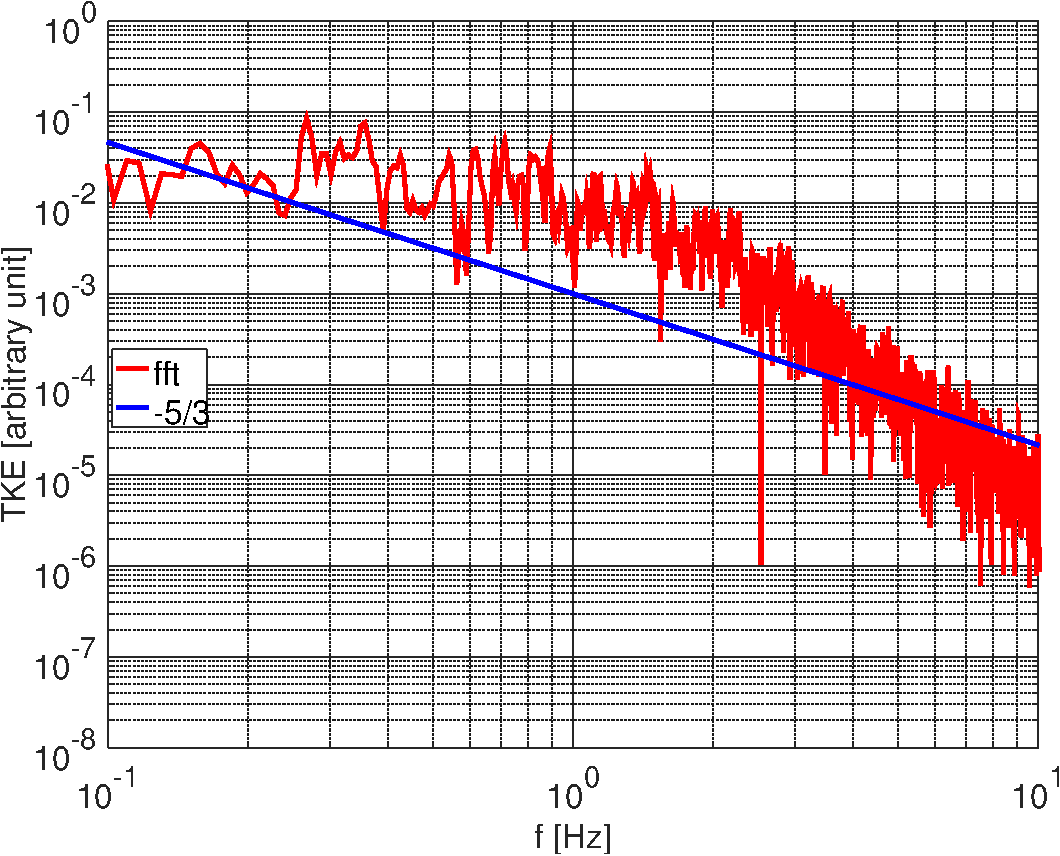
\includegraphics[width=0.95\textwidth]{\orig/.tmp/../CANAL_DAV/spectre0.pdf}
	Energy spectrum for $x = 0.15m$
\end{minipage}
\begin{minipage}{0.4\textwidth}
		\centering
        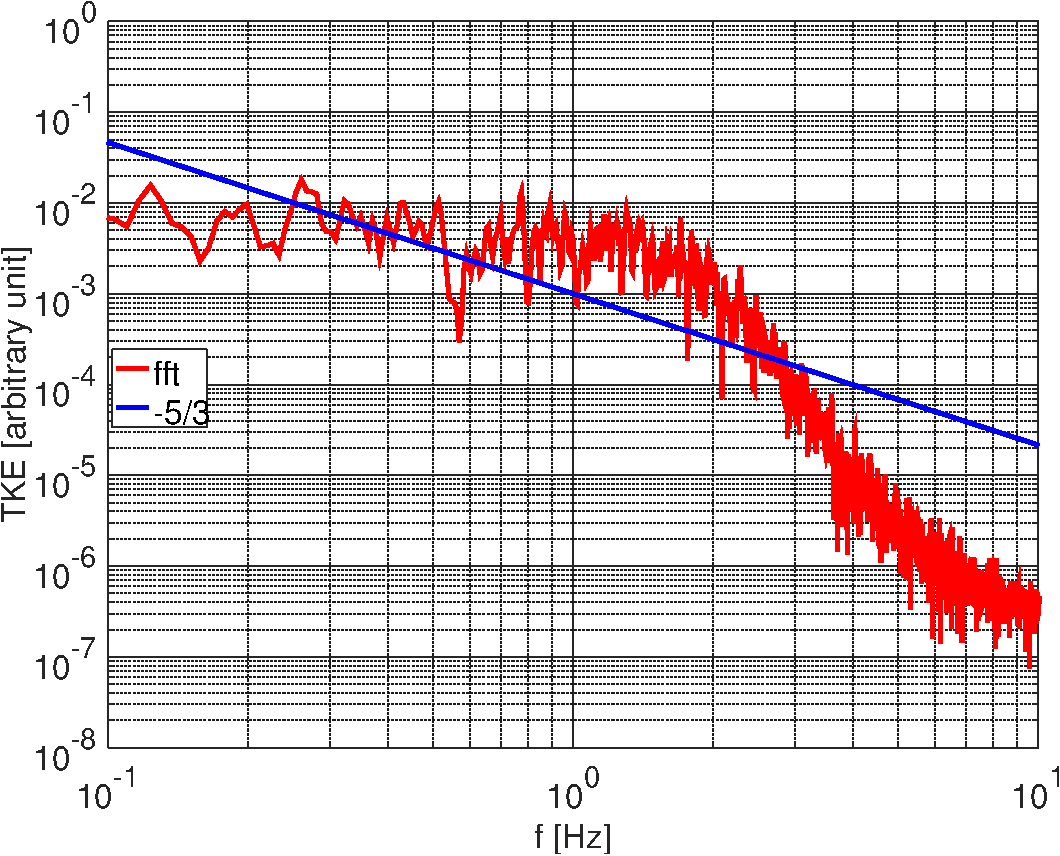
\includegraphics[width=0.95\textwidth]{\orig/.tmp/../CANAL_DAV/spectre10.pdf}
	Energy spectrum for $x = 10m$
\end{minipage}\\
\begin{minipage}{0.4\textwidth}
		\centering
       	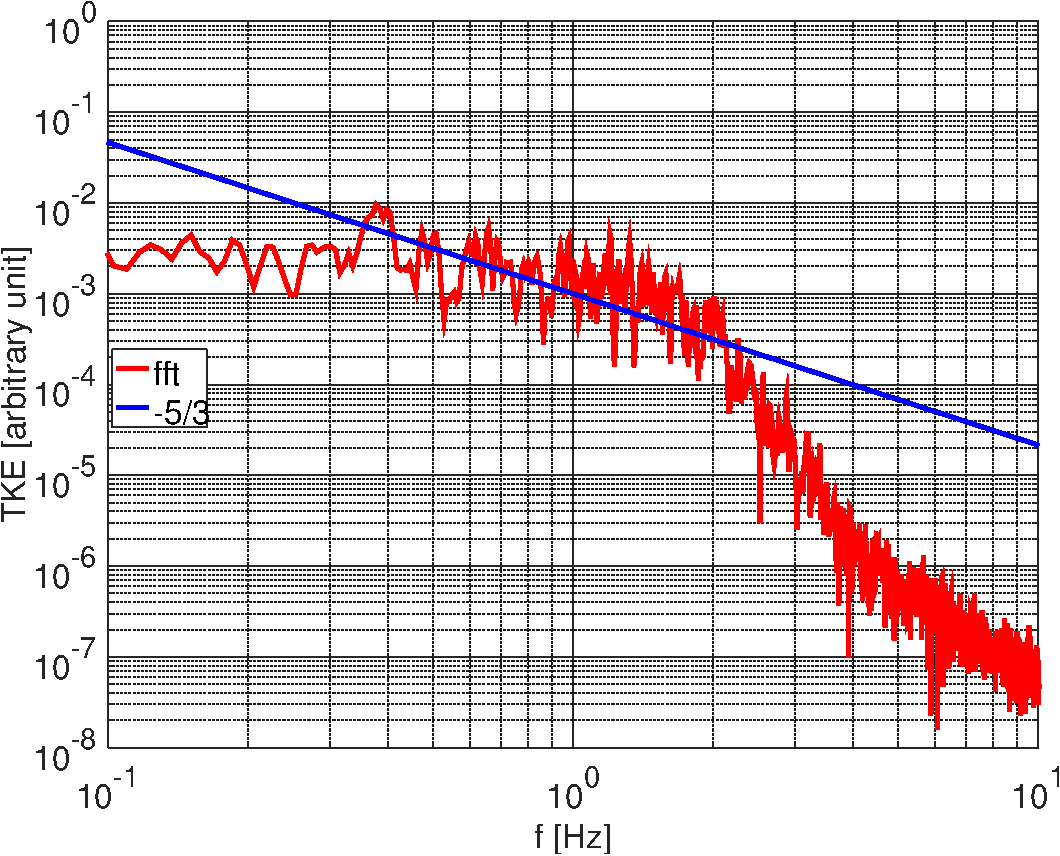
\includegraphics[width=0.95\textwidth]{\orig/.tmp/../CANAL_DAV/spectre25.pdf}
Energy spectrum for $x = 25m$
\end{minipage}
\begin{minipage}{0.4\textwidth}
		\centering
        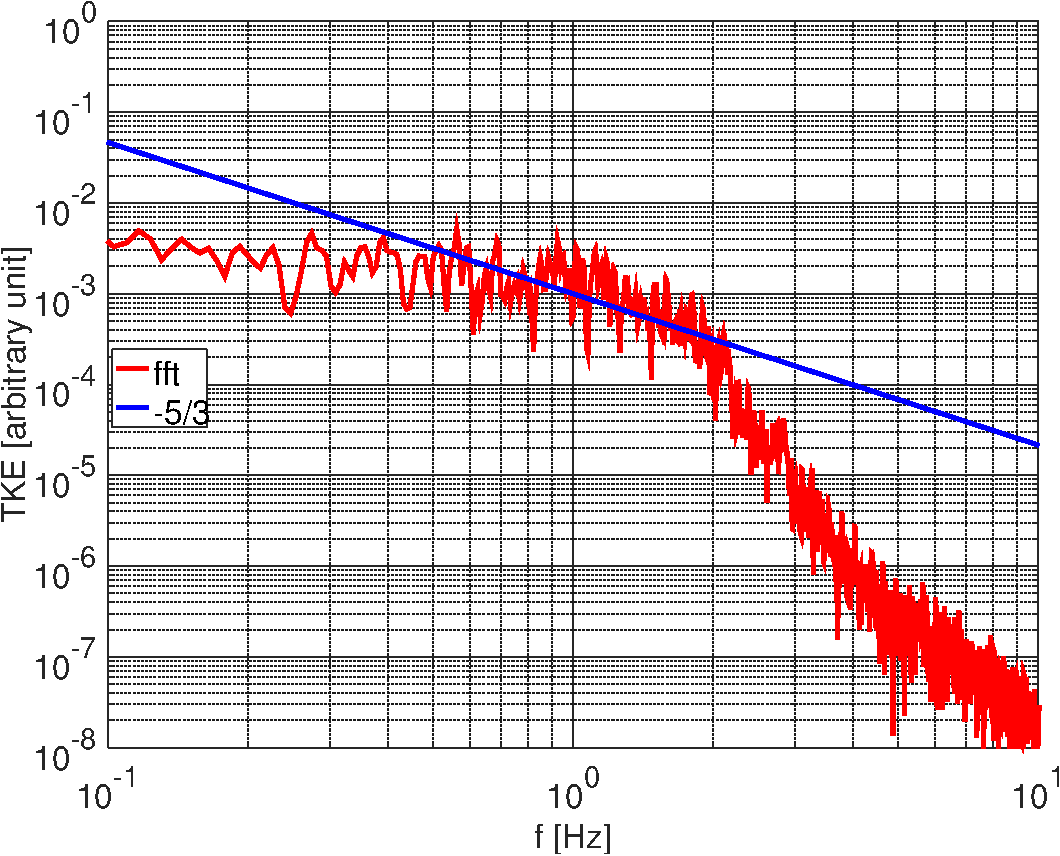
\includegraphics[width=0.95\textwidth]{\orig/.tmp/../CANAL_DAV/spectre30.pdf}
Energy spectrum for $x = 30m$
\end{minipage}\\
\begin{minipage}{0.4\textwidth}
		\centering
        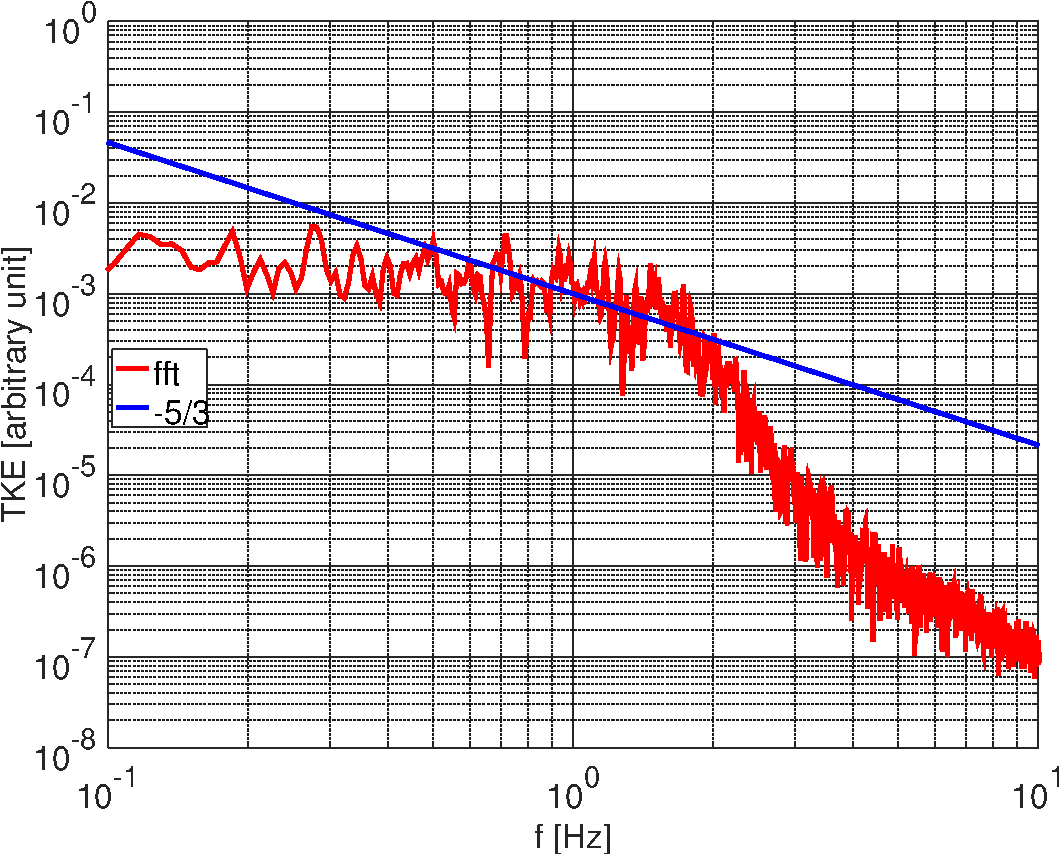
\includegraphics[width=0.95\textwidth]{\orig/.tmp/../CANAL_DAV/spectre40.pdf}
Energy spectrum $x = 40m$
\end{minipage}

